% !TEX root = ../notes_template.tex
\chapter{Appendices}

\section{Mathematical notation} \label{sec:notation}

We strive to use mathematical notation that is consistent with previous publications and across chapters, while also adhering to a few notational conventions.  We generally use:

\begin{enumerate}
    \item Vector-matrix notation, i.e., bold-nonitalic-lowercase for vector (e.g., \(\mathbf{y}\)), bold-nonitalic-uppercase for matrices (e.g., \(\mathbf{Y}\)), and plainface-italic-lowercase for scalars (e.g., \(y\));

    \item Greek symbols (e.g., \(\beta\)) for estimated parameters and Roman symbols (e.g., \(b\)) for data;

    \item Parentheses for indicating the value of a continuous function at a given space and/or time (e.g., \(h(s)\)), and subscripts for indicating the value when the function is being evaluated at a fixed set of modeled locations (e.g., \(h_s\)).
\end{enumerate}
Given these constraints, we typically use the following notation for the following common expressions (Table \ref{tab:Appendix_expression}), variables (Table \ref{tab:Appendix_variables}) and indices (Table \ref{tab:Appendix_indices}).  Individual chapters then augment these conventions, based upon specifics of each topic.  

We note in particular that we use, e.g., \(Y \sim \mathrm{Poisson(\lambda)} \) to indicate that a variable follows the Poisson distribution (or whatever distribution is named on the right-hand-side of an expression), and also use \(\Pr[Y=y] = \mathrm{dPoisson(y|\lambda)}\) for evaluating the probability mass or density function itself.  We will use both notations depending on context, and therefore use both when referring to distributions.   

\begin{table}
  \caption[Notation for commonly used expressions]{A brief summary of common mathematical expressions used throughout the presentation.}
\begin{center}
\begin{tabularx}{\textwidth}{ | X m{4in} | } 
  \hline
  Symbol & Definition \\ 
  \hline
  \( \Pr[X | \theta ]\) & Probability of event \(X\) given parameters \(\theta\), or (using loose notation) the probability density for such an event \\ & \\ 

  \( \mathcal{L}( \theta; Y ) \) & Likelihood for parameters \(\theta\) given data \(Y\) \\ & \\

  \( X \sim \mathrm{Normal}(\mu,\sigma^2) \) & Random variable \(X\) follows a normal distribution with mean \(\mu\) and variance \( \sigma^2 \) \\ & \\

  \( \mathbf{\omega} \sim \mathrm{MVN}(\mathbf{0},\mathbf{\Sigma}) \) & Random vector \( \mathbf{\omega} \) follows a multivariate normal distribution with mean \( \mathbf{0} \) and covariance \( \mathbf{\Sigma} \) \\ & \\

  \( C \sim \mathrm{Poisson}( \lambda ) \) & Count \(C\) follows a Poisson distribution with intensity \( \lambda \) \\ & \\

  \( \Pr[C=c] = \mathrm{dPoisson}( c | \lambda ) \) & The probability that variable \(C\) takes value \(c\) is calculated using a Poisson probability mass function with parameter \( \lambda \) \\ & \\
  
  \( \nabla h(\mathbf{s}) \) & The gradient of a function at location \(\mathbf{s}\), which results in a vector \(\mathbf{v}(s)\) with length equal to the number spatial dimensions \(\mathbf{s}\).  This gradient reduces to a standard derivative calculation (e.g., \( \frac{d}{ds} h(s) \)) when space is defined in one dimension, and is calculated sequentially for each dimension otherwise \\ & \\

  \( \nabla^2 h(s) \) & The Laplace operator of a function \(h\) evaluated at location \(\mathbf{s}\), representing curvature in \(h\) around that location.  This Laplace operator reduces to the standard second-derivative calculation (e.g., \( \frac{d^2}{ds^2} h(s) \)) when space is defined in one dimension.  Otherwise, it is calculated as the sum of second partial derivatives for each individual dimension (\textit{unmixed partial derivatives}):

\begin{equation}
    \nabla^2 h(\mathbf{s}) = \sum_{i=1}^{n} \frac{\partial^2}{\partial s_i^2} h(\mathbf{s})
\end{equation}

  where \(n\) is the number of dimensions involved. \\ & \\

  \( \mathbf{u} \cdot \mathbf{v} \) & The dot-product \(\mathbf{u} \cdot \mathbf{v}\) of two vectors \(\mathbf{u}\) and \(\mathbf{v}\) is calculated by taking the sum of the product of each dimension individually, \( \mathbf{u} \cdot \mathbf{v} = \sum_{s=1}^{n_s} u_s v_s \) where \(n_s\) is the length of each vector.  This arises, e.g., when calculating the dot-product \( \mathbf{v}(s) \cdot \nabla d(s,t) \) of a gradient field \(\nabla d(s,t)\) and an estimated response in each dimension \( \mathbf{v}(s) \) \\

  \hline
\end{tabularx}
  \label{tab:Appendix_expression}
\end{center}
\end{table}

\begin{table}
  \caption[Notation for commonly used variables]{A partial list of symbols used for common variables, quantities, or functions.}
\begin{center}
\begin{tabularx}{\textwidth}{ | X m{4in} | } 
  \hline
  Symbol & Definition \\ 
  \hline
  \( \mathbf{\Sigma} \) & Spatial covariance matrix \\ & \\ 

  \( \mathbf{V} \) & Covariance for non-spatial variables, e.g., among individuals or species \\ & \\ 

  \( \mathbf{Q} \) & Precision (inverse covariance) matrix \\ & \\ 

  \( d_{s,t} \) &  Population density at location \(s\) in time \(t\) \\ & \\

  \( \pi(s) \) &  Sampling or inclusion probability density, i.e., the relative probability that location \(s\) will have a sample available \\ & \\

  \( \beta_t \) & Variable indexed over time (i.e., temporal main effect in GLMM)  \\ & \\ 

  \( \omega_{s} \) & Variable correlated across space (i.e., spatial main effect in GLMM) \\ & \\

  \( \epsilon_{s,t}\) & Variable correlated across space and time (i.e., spatio-temporal interaction in GLMM) \\ & \\

  \( S_j(t) \) & Random variable representing location for individual \(j\) at time \(t\) \\ & \\

  \( \mathcal{D} \) & The spatial domain for which a model is defined, \(s \in \mathcal{D}\) \\ & \\
  
  \( \delta \) & Random variable drawn from a normal distribution, i.e., representing variation in location over time \\ & \\

  \( \Delta_t \) & A specified time-interval used when discretizing time \\ & \\

  \( \Delta_s \) & A specified distance used when discretizing space \\ & \\

  \( \mathbf A \) & Adjacency matrix, representing whether two spatial cells share an edge, where instantaneous movement is nonzero only for adjacent cells \\ & \\

  \(h(S)\) and \(h_s\) & Habitat preference function either defined continuously across space \( h(S) \) or discretized on a grid \(h_s\) \\ & \\

  \( \mathbf{\Lambda} \) & Estimated loadings matrix, representing some subset of columns of the Cholesky matrix associated with covariance \( \mathbf{\Sigma = \Lambda \Lambda}^t \) \\ & \\

  \( g(\mu) = \mathrm{X \gamma} \) & Link function \(g\) used to transform the continuous and unbounded domain of a linear predictor \( \mathrm{X \gamma} \) to the domain for the central tendency \(\mu\) of a random variable \\  

  \hline
\end{tabularx}
  \label{tab:Appendix_variables}
\end{center}
\end{table}

\begin{table}
  \caption[Notation for commonly used indices]{A list of symbols used when indexing elements from a matrix or array.}
\begin{center}
\begin{tabularx}{\textwidth}{ | X m{4in} | } 
  \hline
  Symbol & Definition \\ 
  \hline
  \( s \) & Location of sample or event \\ & \\ 

  \( g \) & Location used for new prediction, e.g., approximating an integral using integration points \\ & \\ 

  \( t \) & Time \\ & \\

  \( c \) & Category in a multivariate model (e.g., species) \\ & \\

  \( i \) & Sample \\ & \\

  \( j \) & Individual \\ & \\

  \( k \) & Covariate \\ & \\

  \( l \) & Factor \\ & \\

  \( m \) & Ancestor \\ 
\hline
\end{tabularx}
  \label{tab:Appendix_indices}
\end{center}
\end{table}

\section{Common Link Functions and Distributions} \label{sec:Appendix_links_and_distributions}

We believe that ecologists are broadly familiar with Generalized Linear Models (GLMs) (see Section \ref{sec:Chap1_GLM}), and therefore typically discuss spatio-temporal models using a vocabulary associated with GLMs. In this vocabulary, measurement \(y_i\) for each sample \(i\) is assumed to follow a distribution with mean \(\mu_i\), and this mean in turn is calculated by applying an inverse-link function \(g^{-1}\) to a linear predictor \(p_i\) that is calculated by adding together some linear transformation of estimated fixed and random effects.   

\begin{equation}
\begin{gathered}
  y_i \sim f( \mu_i, \sigma^2 ) \\
  g(\mu_i) = p_i
\end{gathered}
\end{equation}
We therefore provide a brief summary of common link functions (Table \ref{tab:Appendix_link_functions}) and distributions (Table \ref{tab:Appendix_distributions}).  We acknowledge that there are many more distributions and link functions that are useful and convenient, but restrict attention to those that arise in the main text.  

\begin{table}
  \caption[List of common link functions]{A brief summary of common link functions used when specifying a generalized linear model, where \(\mu\) is the central tendency parameter used subsequently in a probability distribution and \(p_i\) is the linear predictor computed from fixed and random effects.}
\begin{center}
\begin{tabularx}{\textwidth}{ | X X X m{2in} | } 
  \hline
  Link function & Syntax & Inverse-link & Interpretation \\ 
  \hline

  log & \(\mathrm{log}(\mu) = p \) &  \( \mu = e^{p} \) & Constrains \(\mu\) to be positive, and is therefore appropriate when modelling population densities \\ & & & \\ 

  logit & \(\mathrm{logit}(\mu) = p \) &  \( \mu = \frac{e^{p}}{1+e^{p}} \) & Constrains \(\mu\) to be between 0 and 1 (i.e., the range for modelling the probability of an event) in a way that is symmetric \\ & & & \\ 

  Complementary log-log & \(\mathrm{cloglog}(\mu) = p \) &  \( \mu = 1-e^{-e^{p}} \) & Constrains \(\mu\) to be between 0 and 1 in a way that is nonsymmetric and specifically mimics the probability that a count greater than zero arises from a Poisson distribution:
  \begin{equation}
  \begin{gathered}
      C \sim \mathrm{Poisson}(\lambda) \\
      \mathrm{log}(\lambda) = p
  \end{gathered}
  \end{equation}
  where \( \mathrm{Pr}(C > 0) = 1-e^{-\lambda} \) and hence \( \mathrm{cloglog}(\mathrm{Pr}(C > 0)) = p \)  \\ 
 
  \hline
\end{tabularx}
  \label{tab:Appendix_link_functions}
\end{center}
\end{table}

\begin{table}
  \caption[List of common distributions]{A brief summary of common distributions for use in generalized linear models, where \(Y\) is the resulting random variable, \(\mu\) is the central tendency parameter used subsequently in a probability distribution, and other parameters are defined.}
\begin{center}
\begin{tabularx}{\textwidth}{ | X m{1.5in} X m{2in} | } 
  \hline
  Distribution & Syntax & Range & Interpretation \\ 
  \hline

  Normal & \( Y \sim \mathrm{Normal}(\mu,\sigma^2) \) & \( -\infty < Y < \infty \) & Response arises as the sum of many different processes that cumulatively have mean \(\mu\) and variance \(\sigma^2\) \\ & & & \\

  Bernoulli & \( Y \sim \mathrm{Bernoulli}(\mu) \) & \(Y \in \{0,1\} \) & \(\mathrm{Pr}(Y=1) = \mu\) and \(\mathrm{Pr}(Y=0) = 1-\mu\) \\ & & & \\

  Binomial & \( Y \sim \mathrm{Binomial}(N,\mu) \) & \(Y \in \{0,1,...,N\} \) & Response arises as the sum from \(N\) independent Bernoulli distributions each having probability \(\mu\) \\ & & & \\

  Poisson & \( Y \sim \mathrm{Poisson}(\mu) \) & \(Y \in \{0,1,2,...\} \) & Response arises from a Binomial distribution with a very large size \(N\) and low probability for each, where \(\mu = \pi N \) \\ & & & \\

  Gamma & \( Y \sim \mathrm{Gamma}(\sigma^{-2},\mu \sigma^2) \) & \( Y > 0 \) & Response is continuous and positive (e.g., animal size) with mean \(\mu\) and coefficient of variation \( \sigma =  \frac{\sqrt{\mathrm{Var}(Y)}}{\mathrm{Mean}(Y)} \), using shape \(\sigma^{-2}\) and scale \(\mu \sigma^2\) \\ & & & \\

  Lognormal & \( \mathrm{log}(Y) \sim \mathrm{Normal}( \mu,\sigma^2 ) \) & \( Y > 0 \) & Response is continuous and positive, with mean \(\E(Y)=e^{\mu+0.5\sigma^2}\) and coefficient of variation \( \frac{\sqrt{\mathrm{Var}(Y)}}{\mathrm{Mean}(Y)} = \sqrt{e^{\sigma^2}-1} \), using meanlog \(\mu\) and sdlog \(\sigma\), where the lognormal distribution has more density in the tails than the gamma distribution \\ & & & \\

  Tweedie & \( Y \sim \mathrm{Tweedie}( \mu, \phi, \psi ) \)  & \( Y \geq 0 \) & Response is continuous and positive but also has some density at \(Y=0\), where this latter is not within the range of the lognormal or gamma distributions. The variance \(\mathrm{Var}(Y) = \phi \mu^{\psi}\), where \( 1 < \psi < 2 \), and the Tweedie can be interpreted as arising from a compound Poisson-gamma distribution \\ 
  \hline

\end{tabularx}
  \label{tab:Appendix_distributions}
\end{center}
\end{table}

\section{Rejection Sampling} \label{sec:rejection_sampling}

We use \myindex{rejection sampling} to sample values from low-dimensional functions.  It typically becomes less efficient for a higher number of dimensions, and therefore doesn't have as much practical use for higher dimensions (e.g., integrating across random effects).  Rejection sampling seeks to generate samples from a function \(f(x)\), called the ``target distribution".  To do so:
\begin{enumerate}
  \item Calculate the maximum \(M=\mathrm{argmax}_x(f(x))\) of the target distribution;

  \item Draw a sample \(x^*\) from a function \(g(x)\), which is called the ``proposal distribution";

  \item Evaluate the target and proposal distribution at that sample, \(F=f(x^*)\) and \(G=g(x^*)\);

  \item Calculate the ``acceptance probability", \(P=F/(MG)\);

  \item Draw a sample \(p^*\) from a uniform distribution from 0 to 1;

  \item If the uniform sample is less than the acceptance probability, \(p^*<P\), accept and record the sample \(x^*\) or otherwise reject it;

  \item Repeat steps 2 through 6 until the desired number of samples have been accepted, where a larger number of samples will be a more precise approximation to the target distribution.
\end{enumerate}
In the main text, we typically use a uniform distribution for the proposal distribution, \(g(s)=1\).  Rejection sampling is more efficient (i.e., a smaller fraction of samples are rejected) when the target and proposal distributions are similar, and will be perfectly efficient (i.e., all samples are accepted) when \(g(x)=f(x)\).

\section{Matrix Decomposition} 

In the main text, we introduce models that include covariance across locations \(s\), times \(t\), and species \(c\).  These involve specifying a covariance \(\mathbf{\Sigma}\) or its matrix inverse \(\mathbf{Q = \Sigma}^{-1}\), termed the \myindex{precision matrix}.  Both \(\mathbf{\Sigma}\) and \(\mathbf{Q}\) are square and symmetric with dimension \(n_i \times n_i\), and we here review some techniques that are useful to interpret or efficiently compute these important matrices.

\subsection{Eigendecomposition} \label{sec:Appendix_eigendecomposition}

Arguably the most important technique for decomposing a covariance or precision matrix is the \myindex{eigendecomposition}.  This function is accessible in R using function \colorbox{backcolour}{eigen}, and it returns a matrix of eigenvectors \(\mathbf{V}\) and a vector of eigenvalues \(\mathbf{\lambda}\) defined such that:
\begin{enumerate}
    \item \textit{Decomposition}:  we can reconstitute the original matrix \(\mathbf{\Sigma = V \Lambda V}^{-1} \), where \(\mathbf{\Lambda} = \text{diag}(\mathbf{\lambda}) \) is a diagonal matrix of eigenvalues;   

    \item \textit{Orthogonal and unit-length eigenvectors}: each column of \(\mathbf{V}\) is an eigenvector \(\mathbf{v}_j\), and all eigenvectors are orthogonal and have ``length" of one.  This means that \(\sum_{i=1}^{n_i} v_{i,j_1} v_{i,j_2} = 0\) for any pair of eigenvectors \(\mathbf{v}_{j_1}\) and \(\mathbf{v}_{j_2}\), and \(\sum_{i=1}^{n_i} v_{i,j}^2 = 1 \);

    \item \textit{Ordered eigenvalues}: the eigenvalues are ordered from largest to smallest, i.e., \( \lambda_i > \lambda_{i+1}\) for all \(n_i\). 
\end{enumerate}
The function \colorbox{backcolour}{eigen} becomes very slow as matrix size increases.  For sparse matrices, however, we can instead apply the eigendecomposition using the \colorbox{backcolour}{igraph} package \cite{csardi_igraph_2006}, and this remains computationally feasible.  

In the main text, we use the eigendecomposition in several ways:
\begin{itemize}
    \item \textit{Evaluate convergence}:  fitting a maximum likelihood model using the Laplace approximation involves both inner and outer optimizers (Section \ref{sec:Chap2_GLMM}).  Both optimizers must converge for the model to be fitted, and convergence is assessed by identifying the vector of values that minimizes the joint negative log-likelihood (for the inner optimizer) or the log-marginal likelihood (for the outer optimizer), and that the matrix of second derivatives (the Hessian matrix) evaluated at that vector of values is positive definite.  We can check that the Hessian matrix is positive definite by applying an eigendecomposition and confirming that all eigenvalues are positive.  If any of these eigenvalues are sufficiently close to zero, then the Hessian matrix cannot be inverted and either the Laplace approximation cannot be computed (for the inner optimizer) or the estimation covariance is not defined (for the outer optimizer).  Alternatively, if any of these eigenvalues are negative, then the optimizer did not identify the minimum of the function and was not converged.  Furthermore, we can identify the eigenvalues that are problematic (either zero or negative), and then extract the eigenvectors associated with those problematic eigenvalues.  Those eigenvectors then have a nonzero value for those fixed and/or random effects that are associated with convergence issues, and we can focus our attention on identifying problems for those parameters.  We use these properties to diagnose convergence issues in Section \ref{sec:Chap2_convergence_problems}; 
    
    \item \textit{Visualize basis functions}:  if we have a multivariate normal distribution with a given covariance:

    \begin{equation}
        \mathbf{\omega} \sim \mathrm{MVN}(\mathbf{0,\Sigma})
    \end{equation}

    then can instead express it as a series of normal distributions:
    
    \begin{equation}
        \mathbf{\omega} = \sum_{i=1}^{n_i} \mathbf{v}_i \sqrt{\lambda_i} \delta_i
    \end{equation}
    where each \( \delta_i \sim \mathrm{Normal}(0,1) \) is drawn from a standard normal distribution.  Each eigenvector \(\mathbf{v}_i\) projects a normally distributed error with standard deviation of \(1\) to the domain of the specified covariance, while the square-root of each eigenvalue \(\sqrt{\lambda_i}\) defines the standard deviation for that projected vector.  We use this property extensively in Section \ref{sec:Chap5_irregular_spatial_covariance} (e.g., Fig \ref{fig:Chap5_AR_basis_functions}) to visualize the eigenvectors with spatial basis functions that are contained within a given spatial covariance \(\mathbf{\Sigma}\); 

    \item \textit{Diagonal form}:  the eigendecomposition provides a diagonal form for any matrix.  Given the eigendecomposition of the covariance \(\mathbf{\Sigma = V \Lambda V}^{-1} \), we can then calculate the eigendecomposition of the precision as \(\mathbf{Q = V \Lambda}^{-1} \mathbf{V}^{-1} \), where \(\mathbf{\Lambda}^{-1} = \text{diag}(\mathbf{\lambda}^{-1})\).  This shows that the basis functions \(\mathbf{V}\) of a given process are the same when expressed as a covariance or precision matrix, although the eigenvalues are inverted and also ordered from smallest to largest. In Section \ref{sec:Chap5_irregular_spatial_covariance}, we actually calculate the eigendecomposition of the precision matrix \(\mathbf{Q}\) (which is sparse and hence it is cheaper to calculate the eigendecomposition), and then invert the smallest eigenvalues to extract the basis vectors for a given covariance;  
    
    Similarly, in Section \ref{sec:Chap10_assembling_movement_matrix} we define a continuous-time Markov chain for movement rates with rate matrix \(\dot{\mathbf{M}}\), such that integrated movement \(\mathbf{M}\) over interval \(\Delta_t\) is calculated as \(\mathbf{M} = e^{\dot{\mathbf{M}}\Delta_t}\). Rate matrix \(\dot{\mathbf{M}}\) is typically sparse (i.e., non-zero only for adjacent areas), whereas integrated movement \(\mathbf{M}\) is dense (i.e., animals can move anywhere as long as all areas are connected).  Using this property of diagonal matrices, we can calculate the eigendecomposition of the sparse rate matrix \(\dot{\mathbf{M}} = \mathbf{V \dot{\Lambda} V}^{-1}\) relatively cheaply, and this has the same eigenvectors as the integrated movement matrix \(e^{\dot{\mathbf{M}}\Delta_t} = \mathbf{V \Lambda V}^{-1}\) where \( \lambda_i = e^{\dot{\lambda_i}\Delta_t}\).  The stationary distribution (representing expected long-term habitat utilization) is the basis formed from any eigenvectors with an eigenvalue of 1.  So we can calculate this stationary distribution even for an enormous number of locations by calculating the dominant eigenvectors of the sparse movement rate matrix, e.g., using R function \colorbox{backcolour}{igraph::arpack}. 
\end{itemize}

\subsection{Cholesky Decomposition} \label{sec:Appendix_Cholesky}

We introduce \textit{factor models} in Section \ref{sec:Chap4_factor_model} and use them repeatedly in the book.  Here, we provide a brief background on the Cholesky decomposition, which is one interpretation of these factor models. 

The Cholesky decomposition is available for dense matrices in R using \colorbox{backcolour}{chol}, or using the \colorbox{backcolour}{Matrix} package to access various options for sparse matrices.  Applied to a covariance \(\mathbf{\Sigma}\), it returns a matrix \(\mathbf{L}\) with zeros above the diagonal (i.e., a \textit{lower-triangle matrix}) such that \(\mathbf{\Sigma = LL}^T\). If we have a multivariate normal distribution with a given covariance:

\begin{equation}
    \mathbf{\omega} \sim \mathrm{MVN}(\mathbf{0,\Sigma})
\end{equation}
then can instead express it as a series of normal distributions:
    
\begin{equation}
    \mathbf{\omega} = \mathbf{L \delta}
\end{equation}
where each \( \delta_i \sim \mathrm{Normal}(0,1) \) is drawn from a standard normal distribution.  In TMB we can easily specify an estimated loadings matrix \( \mathbf{L} \) to be lower-triangle, and estimating the product of this with a series of independent and normally distributed errors then yields a random effect that has covariance \(\mathbf{\Sigma = LL}^T\).  

\section{Simultaneous Autoregressive Process}\label{sec:Appendix_SAR}

A \textit{{simultaneous autoregressive (SAR) process}}\index{simultaneous autoregressive process} involves re-arranging a spatial variable or model to express it as a simultaneous equation \cite{ver_hoef_relationship_2018}:

\begin{equation} \label{eq:Appendix_SAR_process}
\begin{aligned}
    \mathbf{x} &= \rho \mathbf{Bx + \epsilon} \\
    \mathbf{\epsilon} &= \mathrm{MVN}( \mathbf{0, \Sigma} )
\end{aligned}
\end{equation}
where matrix \(\mathbf{B}\) represents spatial dependencies in an areal or point-process model, typically calculated from an adjacency matrix.  Subtracting \( \rho \mathbf{Bx} \) from both sides yields:

\begin{equation}
\begin{aligned}
    (\mathbf{I} - \rho \mathbf{B}) \mathbf{x} &= \mathbf{\epsilon} \\
    \mathbf{\epsilon} &= \mathrm{MVN}( \mathbf{0, \Sigma} )
\end{aligned}
\end{equation}
Then multiplying both sides by \(  (\mathbf{I} - \rho \mathbf{B})^{-1} \) yields:

\begin{equation}
\begin{aligned}
    \mathbf{x}  &= (\mathbf{I} - \rho \mathbf{B})^{-1} \mathbf{\epsilon} \\
    \mathbf{\epsilon} &= \mathrm{MVN}( \mathbf{0, \Sigma} )
\end{aligned}
\end{equation}
We can then multiply \( (\mathbf{I} - \rho \mathbf{B})^{-1} \) into the covariance for \( \mathbf{\epsilon} \) to yield:

\begin{equation}
    \mathbf{x} \sim \mathrm{MVN}\left( \mathbf{0}, (\mathbf{I} - \rho \mathbf{B})^{-1} \mathbf{\Sigma} ((\mathbf{I} - \rho \mathbf{B})^{-1})^T ) \right)
\end{equation}
This expression therefore defines the covariance for \(x\):

\begin{equation}  \label{eq:Appendix_SAR_covariance}
    \mathbf{V} = \mathrm{Var}(\mathbf{x}) = (\mathbf{I} - \rho \mathbf{B})^{-1} \mathbf{\Sigma} ((\mathbf{I} - \rho \mathbf{B})^{-1})^T
\end{equation}
Alternatively, the inverse covariance (``precision") can then be computed directly as:

\begin{equation} \label{eq:Appendix_SAR_precision}
    \mathbf{V}^{-1} = (\mathbf{I} - \rho \mathbf{B}) \mathbf{\Sigma}^{-1} (\mathbf{I} - \rho \mathbf{B})^T
\end{equation}
and constructing the precision matrix does not require matrix inversion if \(\Sigma\) is diagonal. 

For example, recall that the state-space Gompertz model defines a 1st-order autoregressive process for \(x_t = \mathrm{log}(b_t) \):

\begin{equation}
\begin{aligned}
    x_t & = 
    \begin{cases}
        \frac{\alpha}{1-\rho^2} + \epsilon_t & \text{if } t=1 \\ 
        \alpha + \rho x_{t-1} + \epsilon_t & \text{if } t>1 
    \end{cases} \\
    \epsilon_t & \sim \mathrm{Normal}( 0, \sigma^2) 
\end{aligned}
\end{equation}
This can then be rewritten as a simultaneous equation:

\begin{equation}
\begin{aligned}
    \mathbf{x} &= \frac{\alpha}{1-\rho^2} + \mathbf{z} \\
    \mathbf{z} &= \rho \mathbf{Bz + \epsilon} \\
    \mathbf{\epsilon} &= \mathrm{MVN}( \mathbf{0, \Sigma} )
\end{aligned}
\end{equation}
where:

\begin{equation} 
    \mathbf{B} = \begin{bmatrix}
    0 & 0 & 0 & 0 \\
    -1 & 0 & 0 & 0 \\
    0 & -1 & 0 & 0 \\
    0 & 0 & -1 & 0 \\
    \end{bmatrix} 
\end{equation}
we can then use the SAR form to construct the precision matrix \( \mathbf{V}^{-1} \) directly from \( \mathbf{B} \) and \( \rho \) using Eq. \ref{eq:Appendix_SAR_precision}, and then plug that into the expression \cite{thorson_importance_2014}:

\begin{equation}
\begin{aligned}
    \mathbf{x} &= \mathbf{z} + \frac{\alpha}{1-\rho^2} \\
    \mathbf{z} &= \mathrm{MVN}( \mathbf{0, V}^{-1} )
\end{aligned}
\end{equation}
Furthermore, we can gain some intuition about the sparsity of \( \mathbf{V}^{-1} \) by seeing that:

\begin{equation} 
    \mathbf{I} - \rho \mathbf{B} = \begin{bmatrix}
    1 & 0 & 0 & 0 \\
    -\rho & 1 & 0 & 0 \\
    0 & -\rho & 1 & 0 \\
    0 & 0 & -\rho & 1 \\
    \end{bmatrix} 
\end{equation}
and

\begin{equation} 
    (\mathbf{I} - \rho \mathbf{B})^T = \begin{bmatrix}
    1 & -\rho & 0 & 0 \\
    0 & 1 & -\rho & 0 \\
    0 & 0 & 1 & -\rho \\
    0 & 0 & 0 & 1 \\
    \end{bmatrix} 
\end{equation}
Assuming that \( \Sigma = \sigma^2 \mathbf{I} \), this then yields:

\begin{equation} 
    (\mathbf{I} - \rho \mathbf{B}) \mathbf{\Sigma}^{-1} ((\mathbf{I} - \rho \mathbf{B})^T) = \sigma^{-2} \begin{bmatrix}
    1 & -\rho & 0 & 0 \\
    -\rho & 1+\rho^2 & -\rho & 0 \\
    0 & -\rho & 1+\rho^2 & -\rho \\
    0 & 0 & -\rho & 1+\rho^2 \\
    \end{bmatrix} 
\end{equation}
where this closely resembles the joint precision presented without derivation in Eq. \ref{eq:Chap3_joint_precision}.  We note however, that the two differ somewhat in the variance of the first term \(x_1\) corresponding to the 1st row of \(\mathbf{V}^{-1}\), due to differences in boundary effects.  Importantly, this construction yields the tri-diagonal structure that was automatically detected by TMB using the conditional form of the Gompertz model (Fig. \ref{fig:Chap3_hessian}).

\section{Matrix Exponential Computation}\label{sec:Appendix_matrix_exponential}

In Chapter \ref{Chap10_movement}, we repeatedly use the matrix exponential operator to solve a discretized movement process.  The matrix exponential arises naturally when solving a differential equation:

\begin{equation} 
    \frac{\partial}{\partial t} \mathbf{n}_t^T = \mathbf{n}_t^T \dot{\mathbf{M}} 
\end{equation}
where this represents a continuous-time Markov Chain with instantaneous transition-rate matrix \(\dot{\mathbf{M}}\) \cite{hanks_continuous-time_2015,thorson_estimating_2021}. The solution is then:

\begin{equation} 
    \mathbf{n}_{t+\Delta_t}^T = \mathbf{n}_t^T e^{\Delta_t \dot{\mathbf{M}}}  
\end{equation}
where this arises from integrating the instantaneous rate from time \(t\) to \(t+\Delta_t\).  

\begin{figure}[!ht]
    \caption[Demonstrating Euler approximation for exponential population growth]{A demonstration of the Euler approximation, applied to the exponential growth function \(\frac{d}{dt}b(t) = rb(t)\) and showing either the known solution \(b(t)=b_0 e^{rt}\) as black line, or the Euler approximation (Eq. \ref{eq:Appendix_Euler_approximation}) with an increasing number of sub-intervals \(N\) as colored lines and dots at the breakpoints between linear segments.}
    \centering
    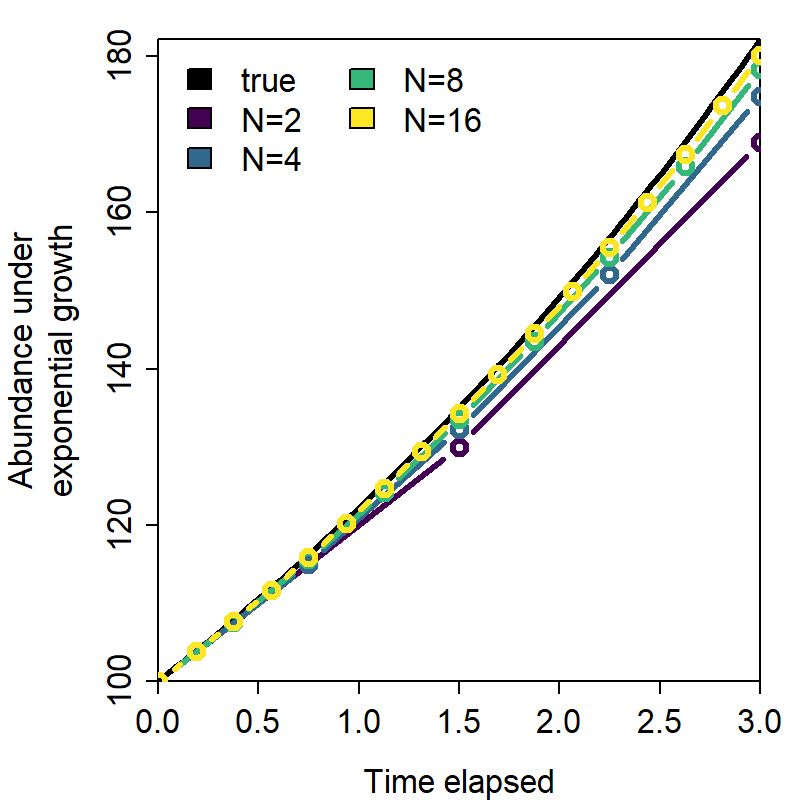
\includegraphics[width=4in]{Appendix/euler_demo.png}
    \label{fig:Appendix_Euler_approximation}
\end{figure}

We highlight three convenient methods for computing this solution in practice:
\begin{enumerate}
    \item \textit{Existing software}:  good statistical software will generally have a matrix exponential function.  We recommend \colorbox{backcolour}{expm::expm} in R, or \colorbox{backblue}{expm} in TMB.  These are generally sufficient when state vector \(\mathbf{n}\) is low-dimensional;

    \item \textit{Euler approximation}:  we introduce the Euler approximation in Eq. \ref{eq:Chap10_euler_approximation}.  There, we claim that it approximates an exponential function with a series of \(N\) linear calculations.  To see this further, we take Eq. \ref{eq:Chap10_euler_approximation}, replace \(\dot{\mathbf{M}}\) with a scalar (intrinsic growth rate \(r\)), and replace vector \(\mathbf{n}\) with a scalar (initial population size \(b_0\)):

    \begin{equation} \label{eq:Appendix_Euler_approximation}
      b(t) = b_0 e^{rt} \approx b_0 \prod_{n=1}^N \left(1+\frac{rt}{N}\right)
    \end{equation}
    We can easily calculate the Euler approximation and visualize how it converges on the true function \(b(t) = b_0 e^{rt}\) as the number of sub-intervals \(N\) increases.  In Fig. \ref{fig:Appendix_Euler_approximation} we can see that even \(N=2\) can roughly approximate the exponential growth function, but higher values of \(N\) approximate the true function more closely.  This same intuition applies to a vector exponential operator, although results with two or more variables are somewhat harder to visualize than the simple one-dimensional example in Fig. \ref{fig:Appendix_Euler_approximation}.

    \item \textit{Uniformization}:  we also introduce \myindex{uniformization} in Section \ref{sec:Chap10_CTMC_cod} without providing any details.  This approach involves calculating the series approximation to the exponential, with the number of series terms set to achieve a desired accuracy.  Recall that the scalar exponential can be approximated as a series:

    \begin{equation} \label{eq:Appendix_series_approximation}
      e^x \approx \sum_{n=0}^N \frac{x^n}{n!}
    \end{equation}
    where \(N\) is set to some sufficiently high number.  We can approximate the matrix exponential using this same series:
    \begin{equation} 
      e^\mathbf{A} \approx \sum_{n=0}^N \frac{\mathbf{A}^n}{n!}
    \end{equation}
    
    If matrix \(\mathbf{A}\) is sparse we can then approximate this summation using a series of sparse matrix calculations, without ever computing \( e^\mathbf{A} \) itself, using a recursive formula:
    \begin{equation} 
      \mathbf{b}^T e^\mathbf{A} \approx \sum_{n=0}^{N} \tilde{\mathbf{b}}_n^T
    \end{equation}

    where:
    \begin{equation} 
      \tilde{\mathbf{b}}_n^T = 
        \begin{cases}
            \mathbf{b}^T & \text{if } n=0 \\ 
            \frac{1}{n} \tilde{\mathbf{b}}_{n-1}^T \mathbf{A} & \text{if } n>0 
        \end{cases} \\
    \end{equation}
    This approach is used in TMB when constructing the object \colorbox{backblue}{expm\_series} using the \colorbox{backblue}{sparse\_matrix\_exponential} library, and it remains computationally efficient even when the number of states is very large.    
\end{enumerate}

